% Copyright (c) 2008-2009 solvethis
% Copyright (c) 2010-2011 Casper Ti. Vector
% Public domain.

\chapter{机器学习类震级预估算法}

\section{神经网络类算法}

\indent 考虑到特征频率和特征幅值两类算法的局限性,本文选取了机器学习中神经网络类算法进行对传统方法进行改进。神经元是构成神经网络最基础的单元,它的结构可抽象成如下图1所示的简单数学模型 (McCulloch and Pitts, 1943),即“M-P神经元模型”。在这个模型中,一个神经元接收到来自n个其他神经元传递过来的输入信号$\mathrm{X}_{\mathrm{i}}$,这些输入信号通过带权重$\mathrm{w}_{\mathrm{i}}$的连接方式进行传递,并将神经元接收到的总输入值$\sum_{i=1}^{n} W_{i} x_{i}$将与神经元的阀值θ进行比较,然后通过“激活函数”处理以产生神经元的输出,这样就完成一个神经元的运算过程。把许多个这样的神经元按一定的层次结构连接起来,就得到各种结构的神经网络。
    
\begin{figure}[!h] 
\centering 
 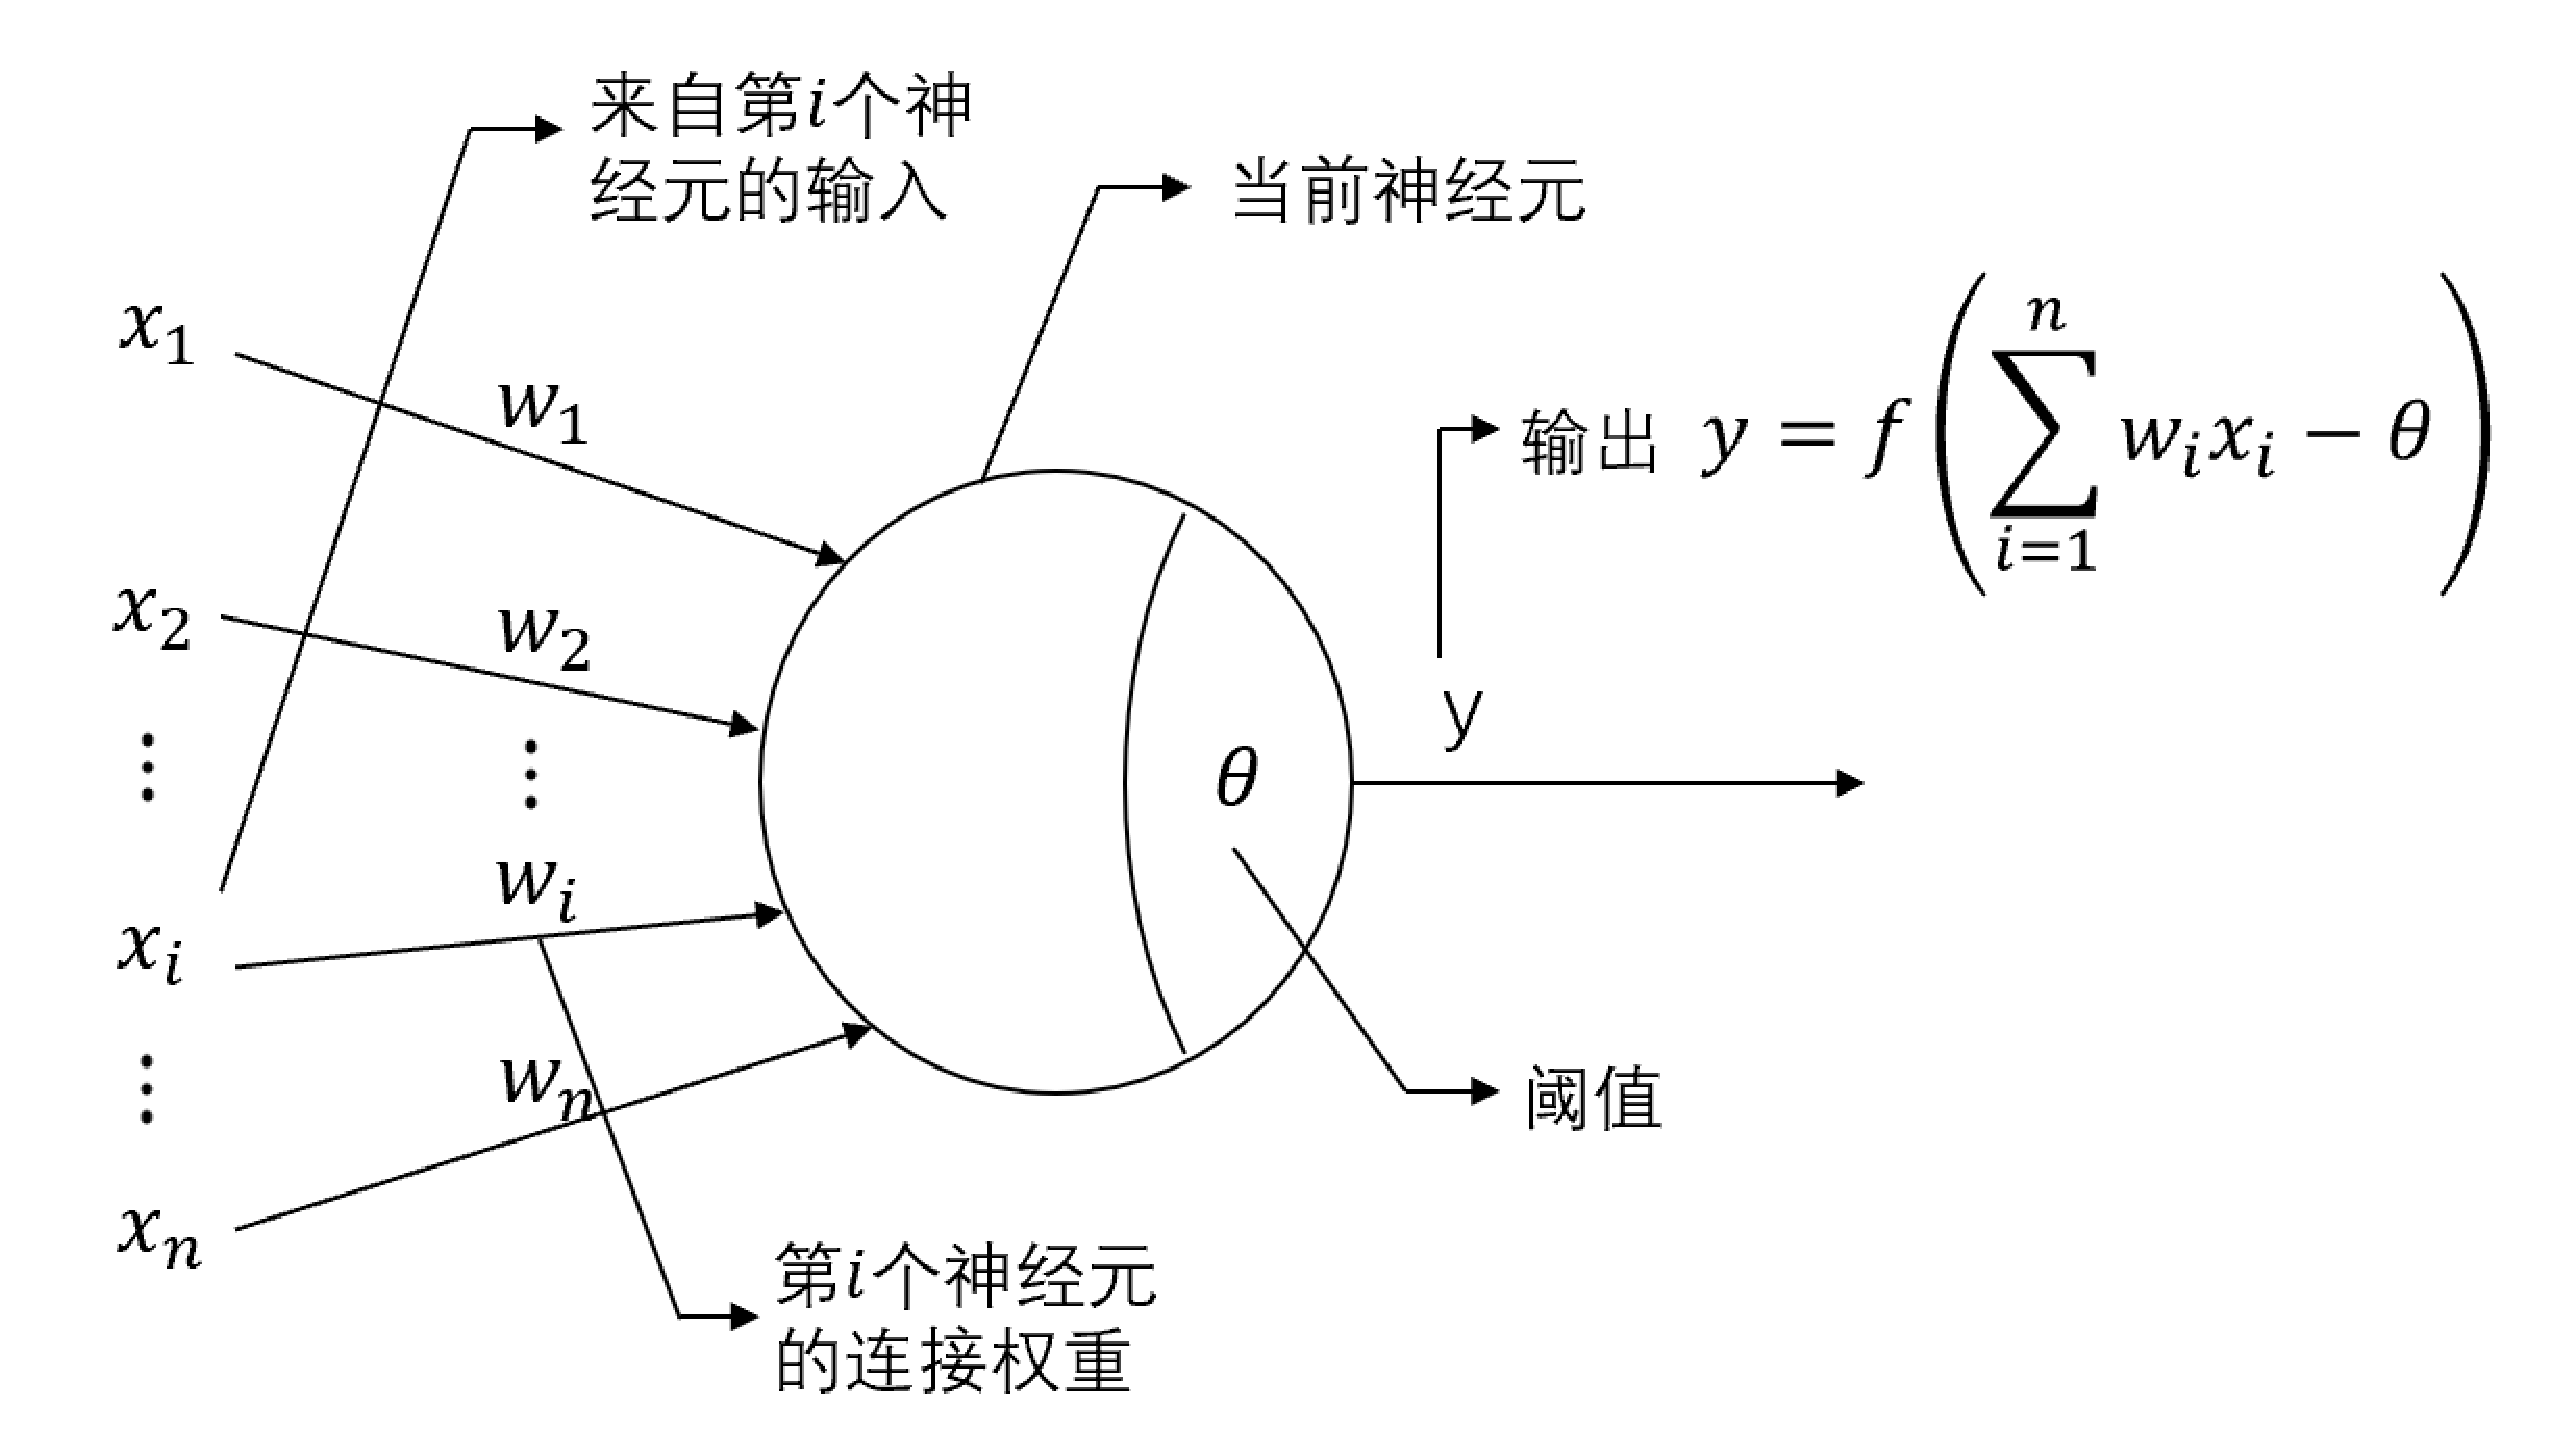
\includegraphics[width=0.7\linewidth]{img/mp.eps} 
 \renewcommand{\figurename}{图} 
\caption{M-P神经元模型示意图} 
%英文标题begin 
\addtocounter{figure}{-1} \vspace{-5pt} 
%\SetEnglishCaption 
\renewcommand{\figurename}{Fig} 
\caption{M-P Neurons model schematic} 
\renewcommand{\figurename}{图} 
%英文标题end 
\label{fig:network-device-influence.png} 
\end{figure}



\section{两类模型的设计}

\indent 我们按照不同训练思路设计出两种神经网络模型用以预估震级。损失函数是机器学习模型效果的评判标准,通过调整模型参数来最小化损失函数以达到优化模型性能的目的。本研究的两种模型的训练目标都按(9)式设置,使用平方误差作为损失函数L。将模型设置为回归问题进行训练,通过(8)式使用BP算法采用梯度下降的方式最小化损失函数以得到优化的神经网络权值$\theta^{*}$(Werbos, 1974; Rumelhart et al., 1986a,b),其中$\mathrm{W}_{\mathrm{i}}$代表第i个隐藏层。同时如下(9)式加入网络权值的$\mathrm{L}_{1}$、$\mathrm{L}_{2}$范数的进行正则约束以防止过拟合。

\begin{equation}
\theta^{*}=\arg \min \frac{1}{N} \sum_{i=1}^{N} L\left(y_{i}, f\left(x_{i} ; \theta_{i}\right)\right)+\sum_{q=1}^{z} \Phi\left(W_{q}\right)
\end{equation}
\begin{equation}
\left\{\begin{array}{c}{L\left(y_{i}, f\left(x_{i}\right)\right)=\left|y_{i}-f\left(x_{i}\right)\right|^{2}} \\ {\Phi\left(W_{q}\right)=\lambda_{1}\left|W_{q}\right|+\lambda_{2} W_{q}^{2}}\end{array}\right.
\end{equation}

其中arg⁡min算符定义为$\theta^{*}=\arg \min f(\theta)$下,使$f(\theta)$达到最小值的$\theta$值,N为采用mini-batch方式每次训练抽样数量的大小,z代表隐藏的层数。

\indent NN模型结构如图2所示,整体框架为全连接神经网络。隐藏层间连接方式为下(10)和(11)式,
\begin{equation}
\mathrm{Z}_{\mathrm{c}}^{i}=\sigma\left(b_{c}^{i}+\sum_{c^{\prime}=1}^{c_{i}} Z_{C^{\prime}}^{i-1} \cdot W_{C C^{\prime}}^{i}\right)
\end{equation}
\begin{equation}
\sigma(x)=\max (0, x)
\end{equation}



其中下角标C,$C^{\prime}$代表了输出层和输入层,上角标i代表第i个隐藏层。激活函数使用(11)式中所示的以0为分界的分段函数ReLU(Alex et al., 2012)。当此激活函数接收到前一隐层小于0的输入时输出0,而当接收到大于0的隐藏层输入时不做处理直接作为输出。NN模型以特征频率类方法的思想为基础,但区别于$\tau_{\mathrm{C}}$方法只使用垂直分量的信息,此NN神经网络的使用台站记录的全三分量信息,以期望得到不同分量联合与破裂规模的关系。将3s时窗内的三分量频谱信息并列为一维张量(tensor)作为模型输入,预估的震级结果作为模型输出。整个模型共有7层神经网络,除去首尾的输入、输出层外共设置5个隐藏层。根据Hinton(2012a,2012b)和Alex(2012),我们在第1和第3隐层后连接Dropout层以防止过拟合,同时加快有效训练速率。

    

\begin{figure}[!h] 
\centering 
 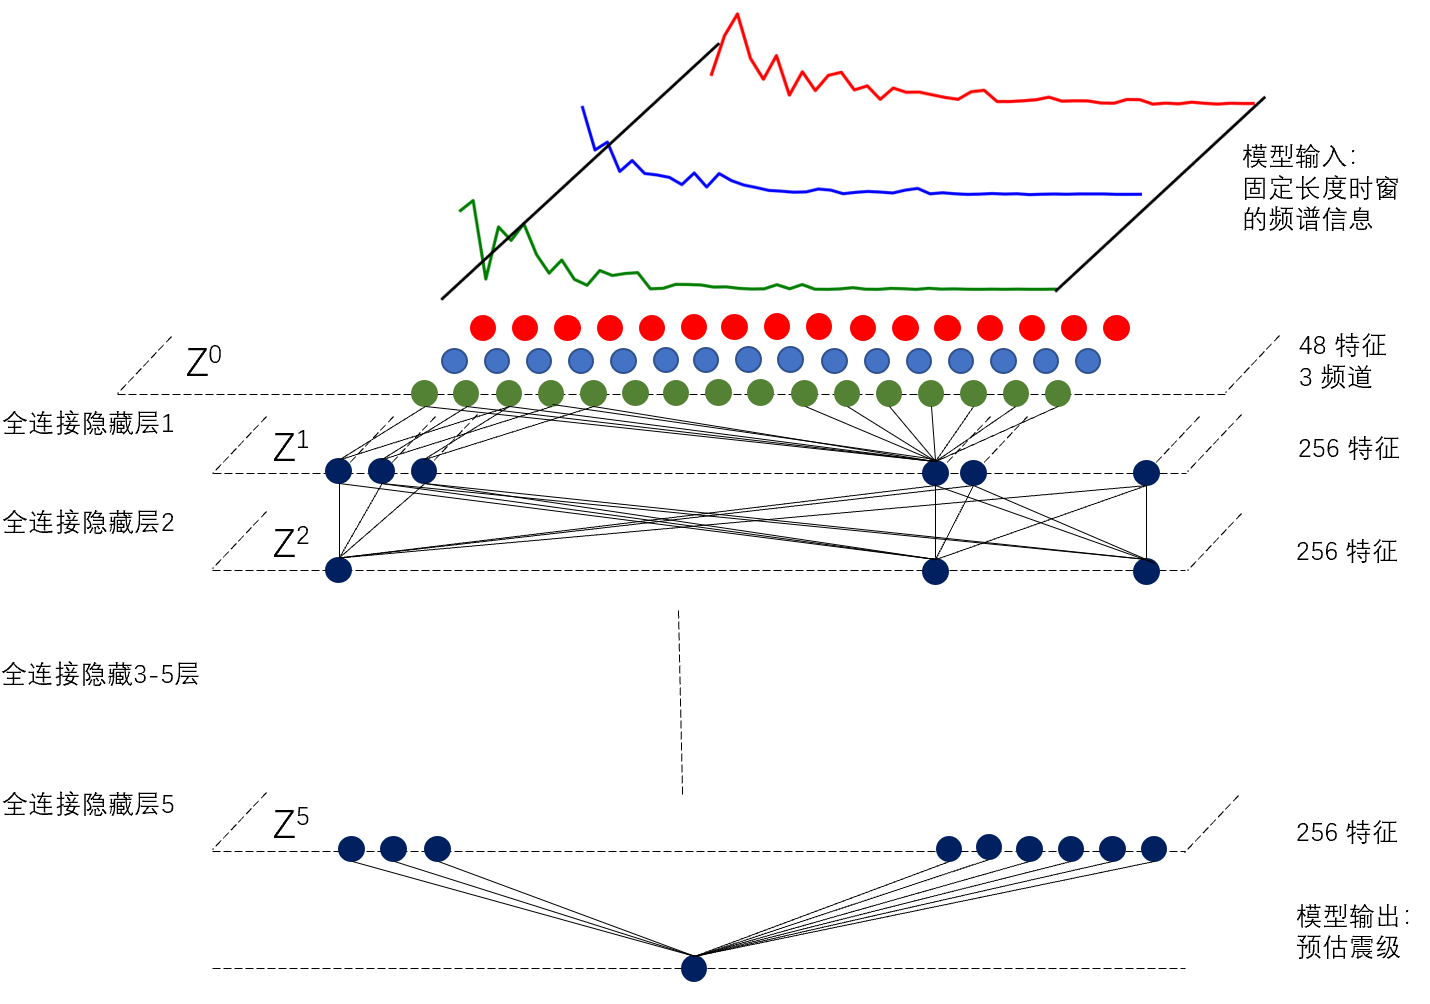
\includegraphics[width=0.99\linewidth]{img/NN.png} 
 \renewcommand{\figurename}{图} 
\caption{NN神经网络结构示意图} 
%英文标题begin 
\addtocounter{figure}{-1} \vspace{-5pt} 
%\SetEnglishCaption 
\renewcommand{\figurename}{Fig} 
\caption{NN neural network mechanism diagram} 
\renewcommand{\figurename}{图} 
%英文标题end 
\label{fig:network-device-influence.png} 
\end{figure}


\begin{figure}[!h] 
\centering 
 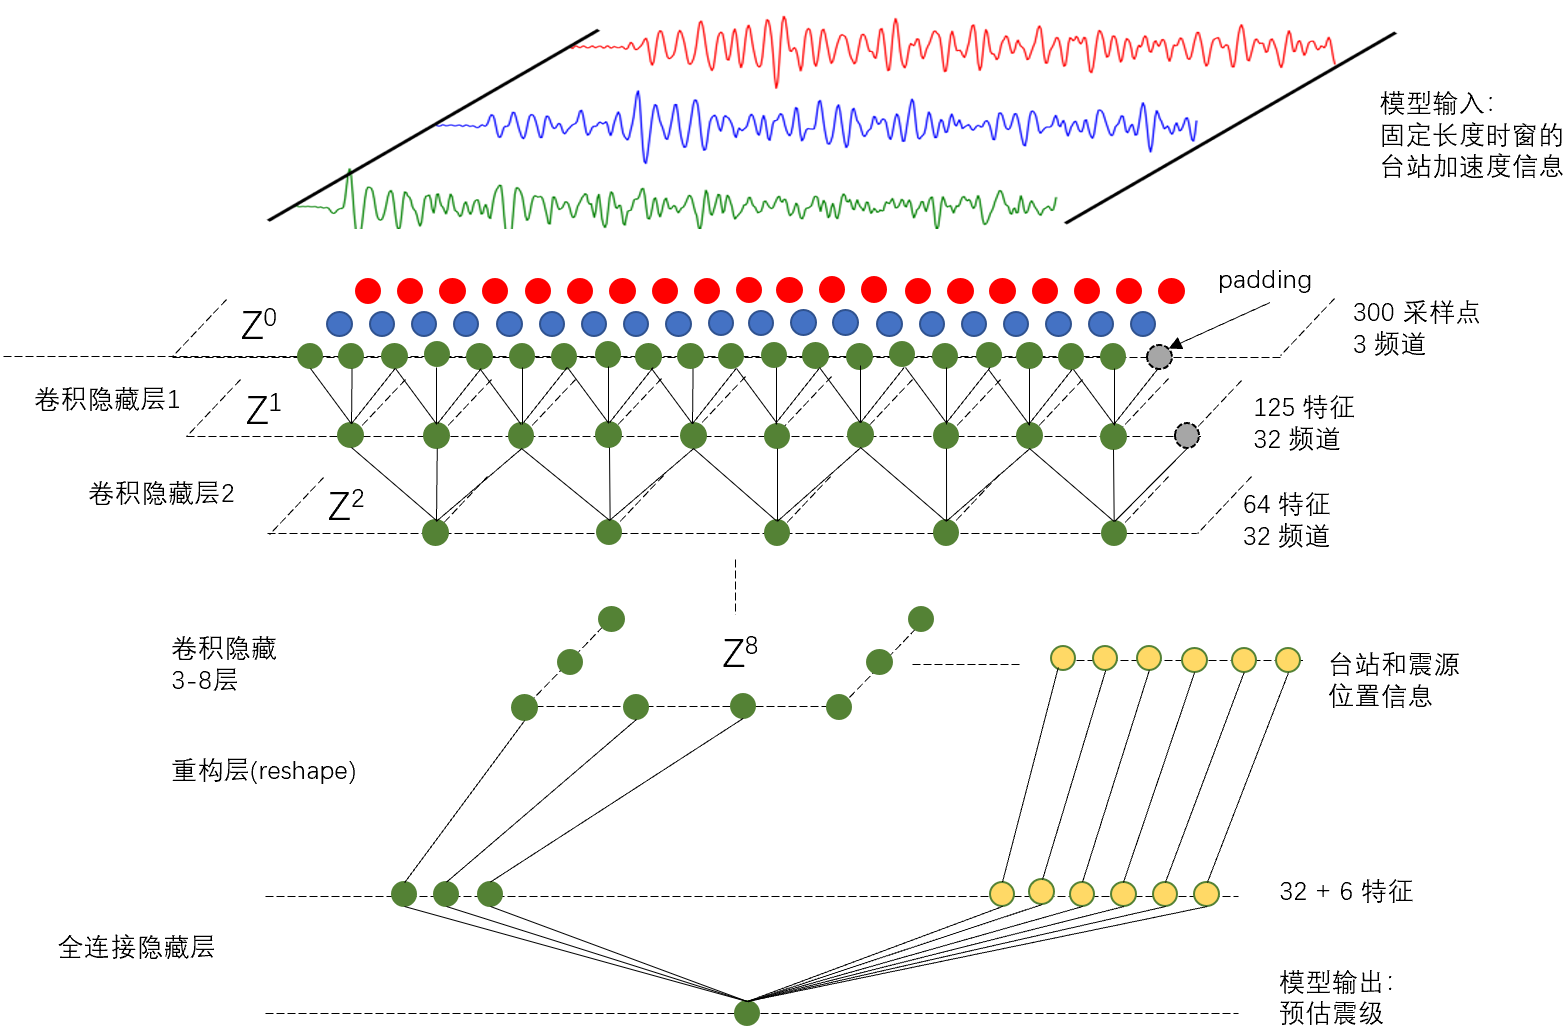
\includegraphics[width=0.99\linewidth]{img/CNN.png} 
 \renewcommand{\figurename}{图} 
\caption{CNN深度神经网络结构示意图} 
%英文标题begin 
\addtocounter{figure}{-1} \vspace{-5pt} 
%\SetEnglishCaption 
\renewcommand{\figurename}{Fig} 
\caption{Schematic diagram of CNN deep neural network structure} 
\renewcommand{\figurename}{图} 
%英文标题end 
\label{fig:network-device-influence.png} 
\end{figure}
\indent CNN模型结构如图3所示,整体框架为CNN卷积神经网络。与NN模型相同,使用ReLU作为激活函数,使用全三分量信息,并仍以预估的震级结果作为模型输出。不同的是,CNN模型将3s时窗内的加速度记录处理为三维张量(tensor)作为模型输入,根据John(2017)并结合本问题的特性,全网络共设置8层卷积层且无池化层设置。卷积层采取小卷积核进行卷积计算,同时采用2个步长的卷积时窗移动以帮助卷积核降采样。卷积隐藏层的运算方式见(10)式。在第8层卷积层后,将所有特征重排列与台站和震中经纬深度信息一同并列后,进行全连接运算输出。考虑到深度学习卓越的表达能力,$\mathbf{\tau}_{\mathrm{c}}$方法中傅里叶变换的预处理是很容易被卷积神经网络完成的,并且还会有更多其他的特征被卷积核提取。\\
\indent 考虑到模型输入的信息量和CNN网络的表达能力,理论上此模型至少可达到$\mathbf{\tau}_{\mathrm{c}}$和$P_{d}$方法的效果。如图3所示,此模型与NN模型相比还引入了台站和震源的位置信息。并且不同于$P_{d}$方法中相对量震中距离的使用,引入台站和震源的坐标信息还在一定程度上可以帮助模型完成区域断层信息、地球介质模型记录,使模型作为区域震级预估方法有更出色的表现。此深度学习模型对原始输入信号进行逐层加工,从而把初始的、与输出目标之间联系不太密切的输入表示,转化成与输出联系更为密切的新表示方式,使得原本难以完成的任务成为可能(对比于NN模型频谱信息输入和最后输出间的映射)。\\
\indent CNN模型端到端的模型设置导致其训练难度更大,也意味着就需要更多的训练数据,由于目前数据量不足暂时还未对CNN模型完成训练。



\section{模型评估与选择}

 \indent 通常上我们把机器学习器在训练集上的误差称为训练误差(training error)或者经验误差(generalization error),在新样本上的误差称为泛化误差(generalization error)。原则上最终人们希望得到一个泛化误差小的模型,也就是模型在面对没有出现在训练集中的新数据能有优异的预测性。但事实上我们并不知道新的样本是什么样的,具体到本问题中对于还未发生的地震我们并不知道其发震断层的模型,也不清楚震源附近的介质模型,实际上能做的是努力使训练误差最小化。在很多情况下,我们都可以使模型学习到一个在训练集上表现很好,经验误差很小的机器学习器。甚至对于整个训练数据集没有错误分类达到100\%准确率或者完全没有预测误差的学习器,但这样的机器学习器在绝大多数的情况下并没有好的泛化能力。\\
 \indent 我们核心的训练目标是在新样本上表现卓越。为了达到这个目的,我们要使模型从训练数据中尽可能的学习到问题"内在规律",这样才能使模型在遇到实时地震台站数据记录时做出正确判别。当学习器把训练样本学得“太好”时,很可能已经把训练样本自身的一些特点当作了所有潜在样本都会具有的一般性质,这就很会导致泛化性能下降。此现象在机器学习中称之为"过拟合"(overfitting),与之相对应“欠拟合”(underfitting),这是指对训练样本的一般性质尚未学习好。图2.4直观展示了过拟合和欠拟合的区别。
 
\begin{figure}[ht]
  \centering
  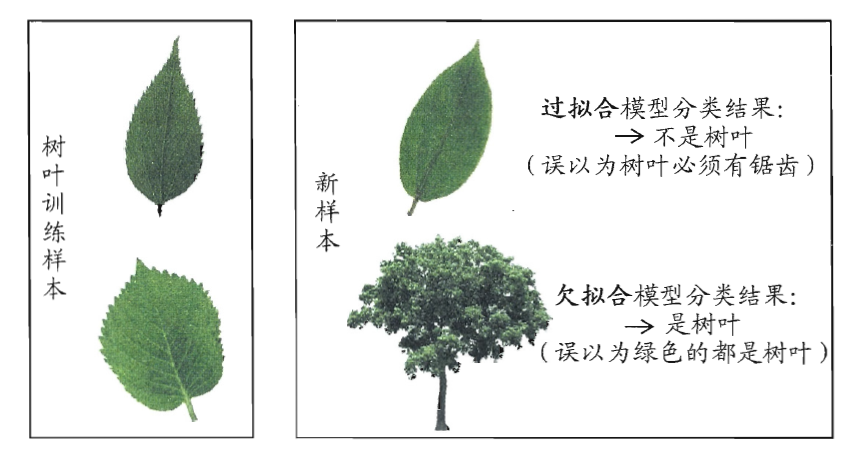
\includegraphics[width=0.8\linewidth]{img/fitting.jpg}
  \caption{过拟合、欠拟合的直观类比}\label{fig:yinglimoxin}
\end{figure}

 \indent 机器学习模型往往着力于解决的过拟合问题。在实践中往往有多种原因导致过拟合问题的出现。较为常见的情况有,因模型学习能力过于强而导致训练数据集中所包含的非一般特性都被模型学习到。而欠拟合则通常是由于模型复杂度低下和学习能力不足造成,例如在神经网络学习中采取增加模型网络深度和增加训练轮数可以克服欠拟合问题。与之相对的过拟合问题是机器学习面临的核心阻碍,在各类具体的机器学习模型中都有各自机制来应对,但原则上过拟合问题是不可避免的,以上的机制也只能部分的缓解过拟合问题。\\
 \indent 一般的可以通过实验测试来对机器学习模型的泛化能力进行评估,同时完成对模型参数的选择。故我们需要一个有别于训练数据集(training set)的测试数据集(testing set)。若假设测试数据集中新样本也是从真实事件分布中独立同分布采样而得到,同时测试数据集与训练数据集互斥度越大越佳,这就意味着测试数据集中样本尽量没有出现过在训练过程中。在这种假设下我们可以使用测试数据集的测试误差(testing error)作为模型对于真实泛化能力的估计。机器学习模型对于新样本的分别能力越出众,则其在测试数据集上的误差越小。对于一个包含m个样本的数据集$D=\left\{\left(\boldsymbol{x}_{1}, y_{1}\right),\left(\boldsymbol{x}_{2}, y_{2}\right), \ldots\right.\left(\boldsymbol{x}_{m}, y_{m}\right) \}$,通常从D中适当的分出训练集S和测试集T两个互斥的子集。\\
 \subsection{朴素留出训练方法}
 \indent 常见朴素的思想以留出法为框架。通常的做法为直接将全数据集D划分为互斥的两个集合,这两个集合S、T满足,$D=S \cup T, S \cap T=\varnothing$. ~即使用训练数据集S上进行模型训练,随后在测试数据集T上进行模型泛化能力评估。\\
 \indent 留出法最核心的问题是需要既要使训练集和测试集分布保持一致性又要使得两个集合足够互斥,这就意味着要尽量避免因为分布带来的问题。例如如果训练数据集与真实分布不一致,则会导致训练出的模型天然有偏差。这就要求假设在面对分类问题时,使用分层采样的方式在不同类别样本上按比例随机采样,保持住训练集和真实分布的一致性。同时考虑到如果测试数据集与真实分布差异过大,显而易见的会使对模型评估的环节变得没有意义,甚至产生负面指导作用。\\
 \indent 朴素留出方法天然面临着无法解决两难的困境。一方面如果训练集S太小,则给予机器学习模型的训练信息不足够充分难以训练出优秀的模型。另一方面我们希望使用测试数据集T测试出机器学习模型对于评估原始数据集D的能力,所以就要求测试数据集T不能太小,使其能够拥有足够多的原始数据D集中的信息。这导致了在往往有限的数据量的情况下,两个互斥的测试集和训练集都有数据量要求。这一矛盾在数据量有限的情况下无法调和,经验上选取原始数据量的60\%至90\%作为训练集S,剩余没用使用的数据样本纳入测试集T。\\
 \subsection{交叉验证法}
 \indent 交叉验证法(cross validation)为了解决朴素留出法难以平衡评估稳定性和保真性的问题,将原始数据集D划分为k个大小相似的互斥子集(也称为k折交叉检验),即$D=D_{1} \cup D_{2} \cup \ldots \cup D_{k}, D_{i} \cap D_{j}=\varnothing(i \neq j)$,每个子集都采取分层采样的方式来保证数据分布一致性。此方法如下图所示,每次选取k-1个数据集的合并作为训练集,剩余一个数据集作为测试集。如上述描述数据集选取方式的使得单一训练过程的训练数据量足够大。为了兼顾模型评估的保真性,我们重复进行k次以上操作,每次的验证集都是之前训练过程所不相同的,共训练出不一样的k个模型,这些模型结果的平均值作为整个系统的输出用于评估。\\
 \indent 可以看出在数据集比较大时,训练k个模型的开销是巨大的。所以交叉验证法在改善了朴素留出法性能问题的同时,也面临着速度和精度的取舍

 \begin{figure}[!h] 
\centering 
 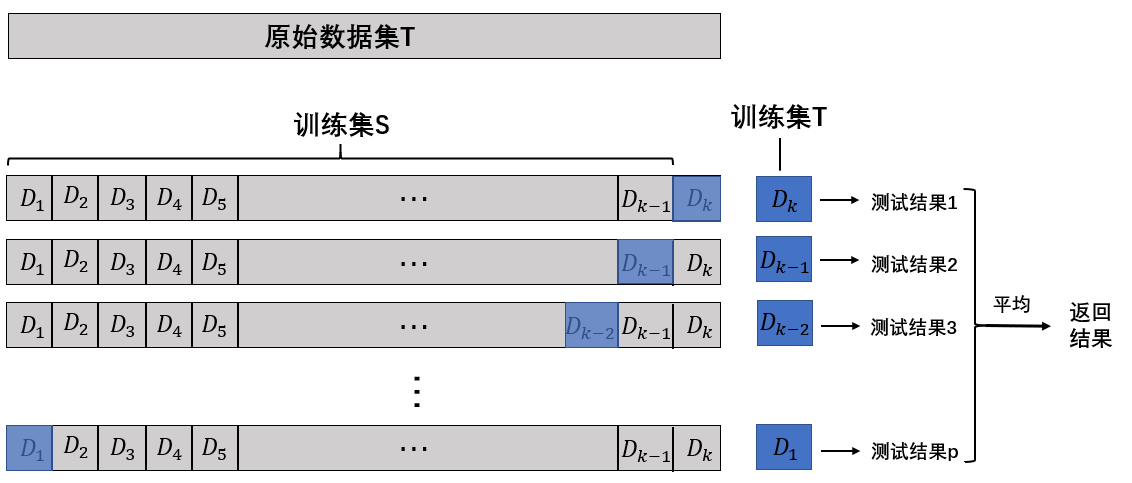
\includegraphics[width=0.95\linewidth]{img/cv.jpg} 
 \renewcommand{\figurename}{图} 
\caption{交叉检验示意图} 
%英文标题begin 
\addtocounter{figure}{-1} \vspace{-5pt} 
%\SetEnglishCaption 
\renewcommand{\figurename}{Fig} 
\caption{Cross-validation diagram} 
\renewcommand{\figurename}{图} 
%英文标题end 
\label{fig:network-device-influence.png} 
\end{figure}
 

\indent 具体到本文研究中,我们结合朴素留出法和交叉验证法将所有的地震记录划分为训练集、交叉验证集和测试集三部分。不同于交叉检验法的多组模型训练,只训练出一组模型\\



 \begin{figure}[h]
  \centering
  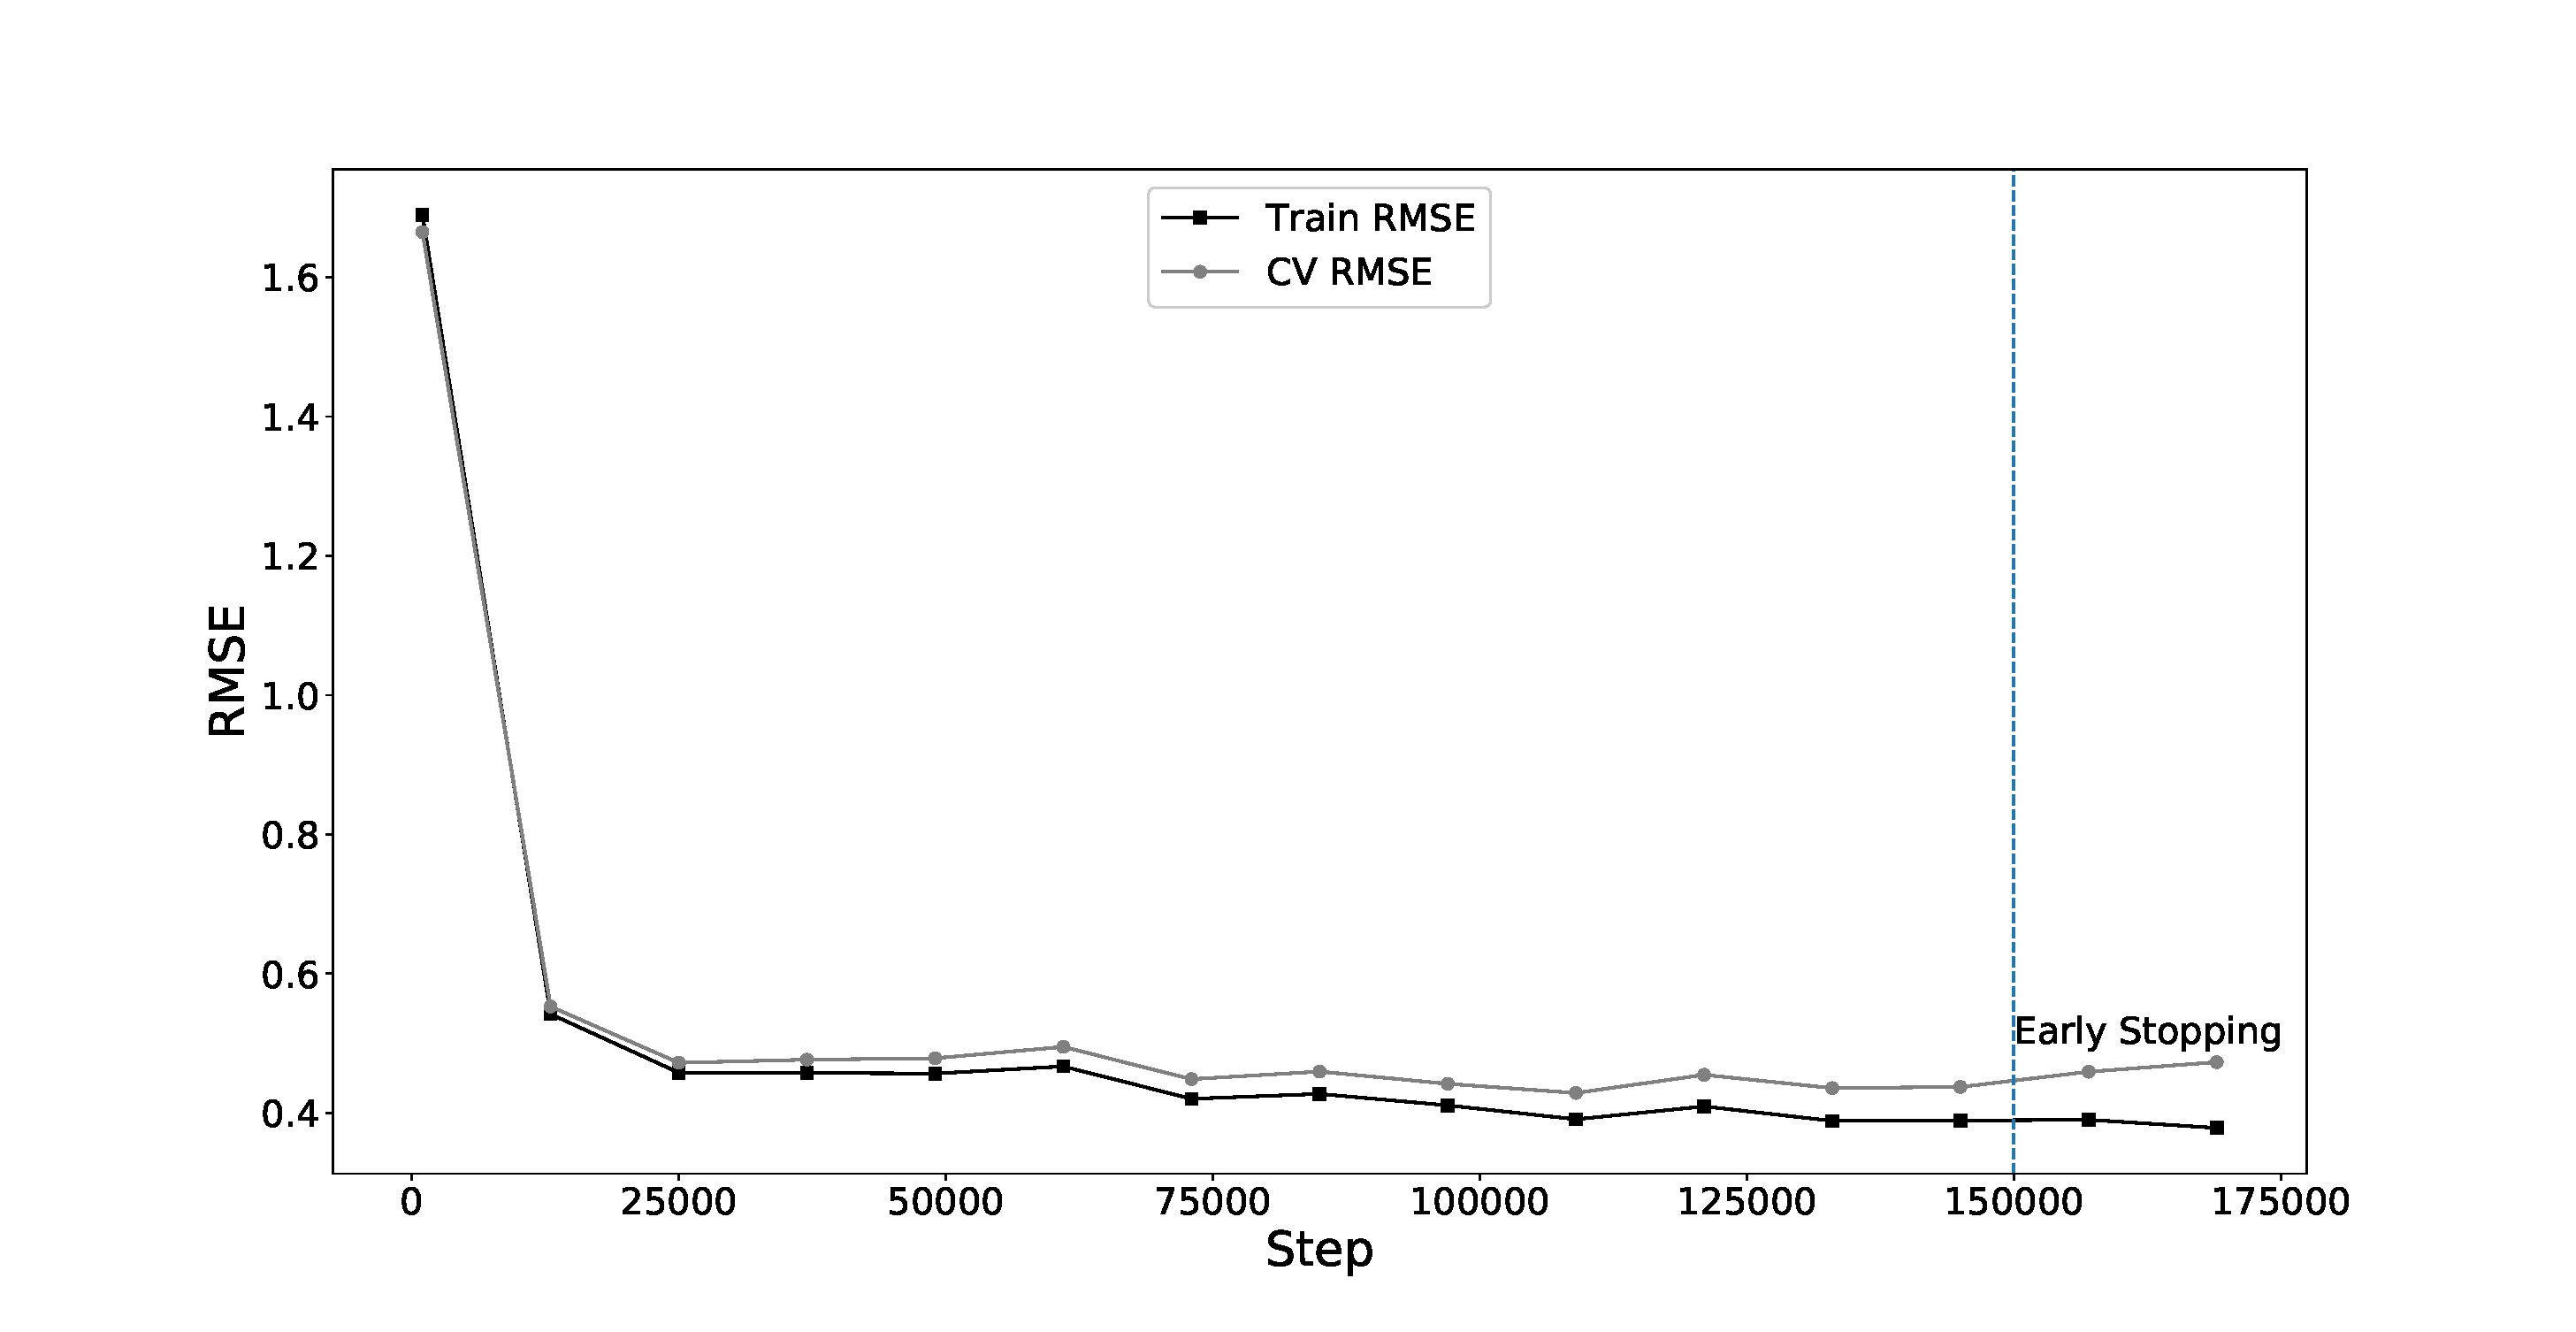
\includegraphics[width=\linewidth]{img/6.eps}
  \caption{K折交叉检验示意图}\label{fig:yinglimoxin}
\end{figure}



\begin{figure}[h]
  \centering
  \begin{subfigure}[b]{0.45\linewidth}
    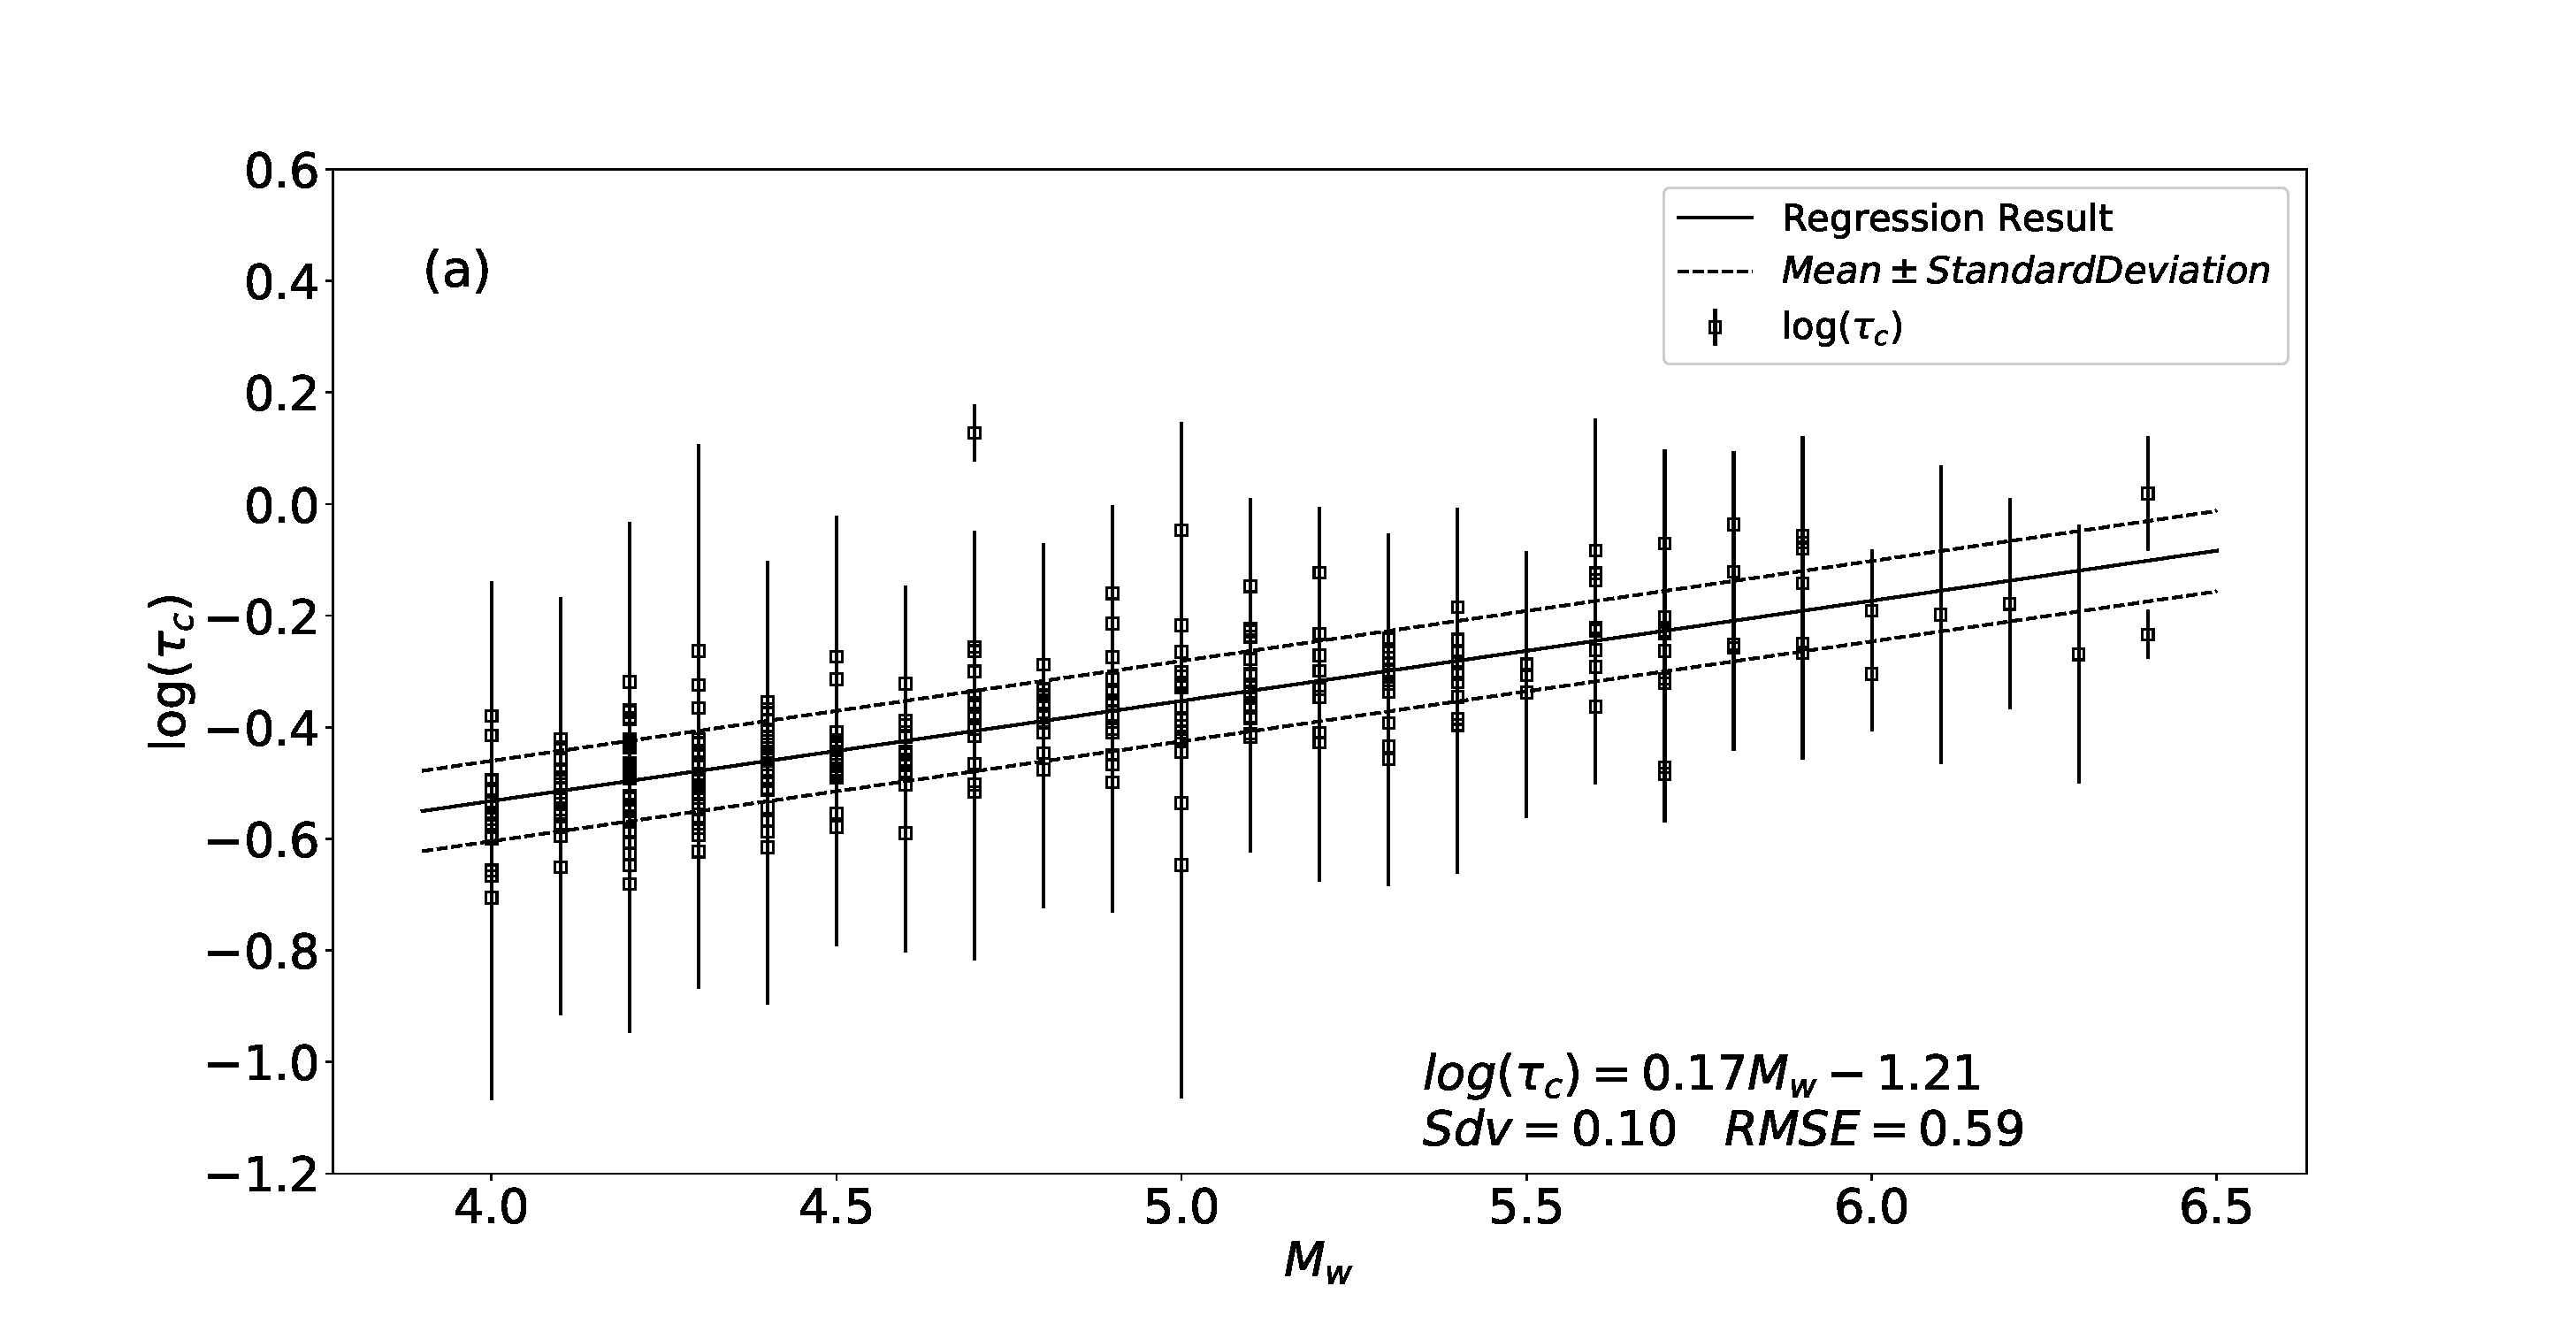
\includegraphics[width=\linewidth]{img/7a.eps}
    \caption{应力传模型}\label{fig:yinglimoxin}
  \end{subfigure}
  \begin{subfigure}[b]{0.45\linewidth}
    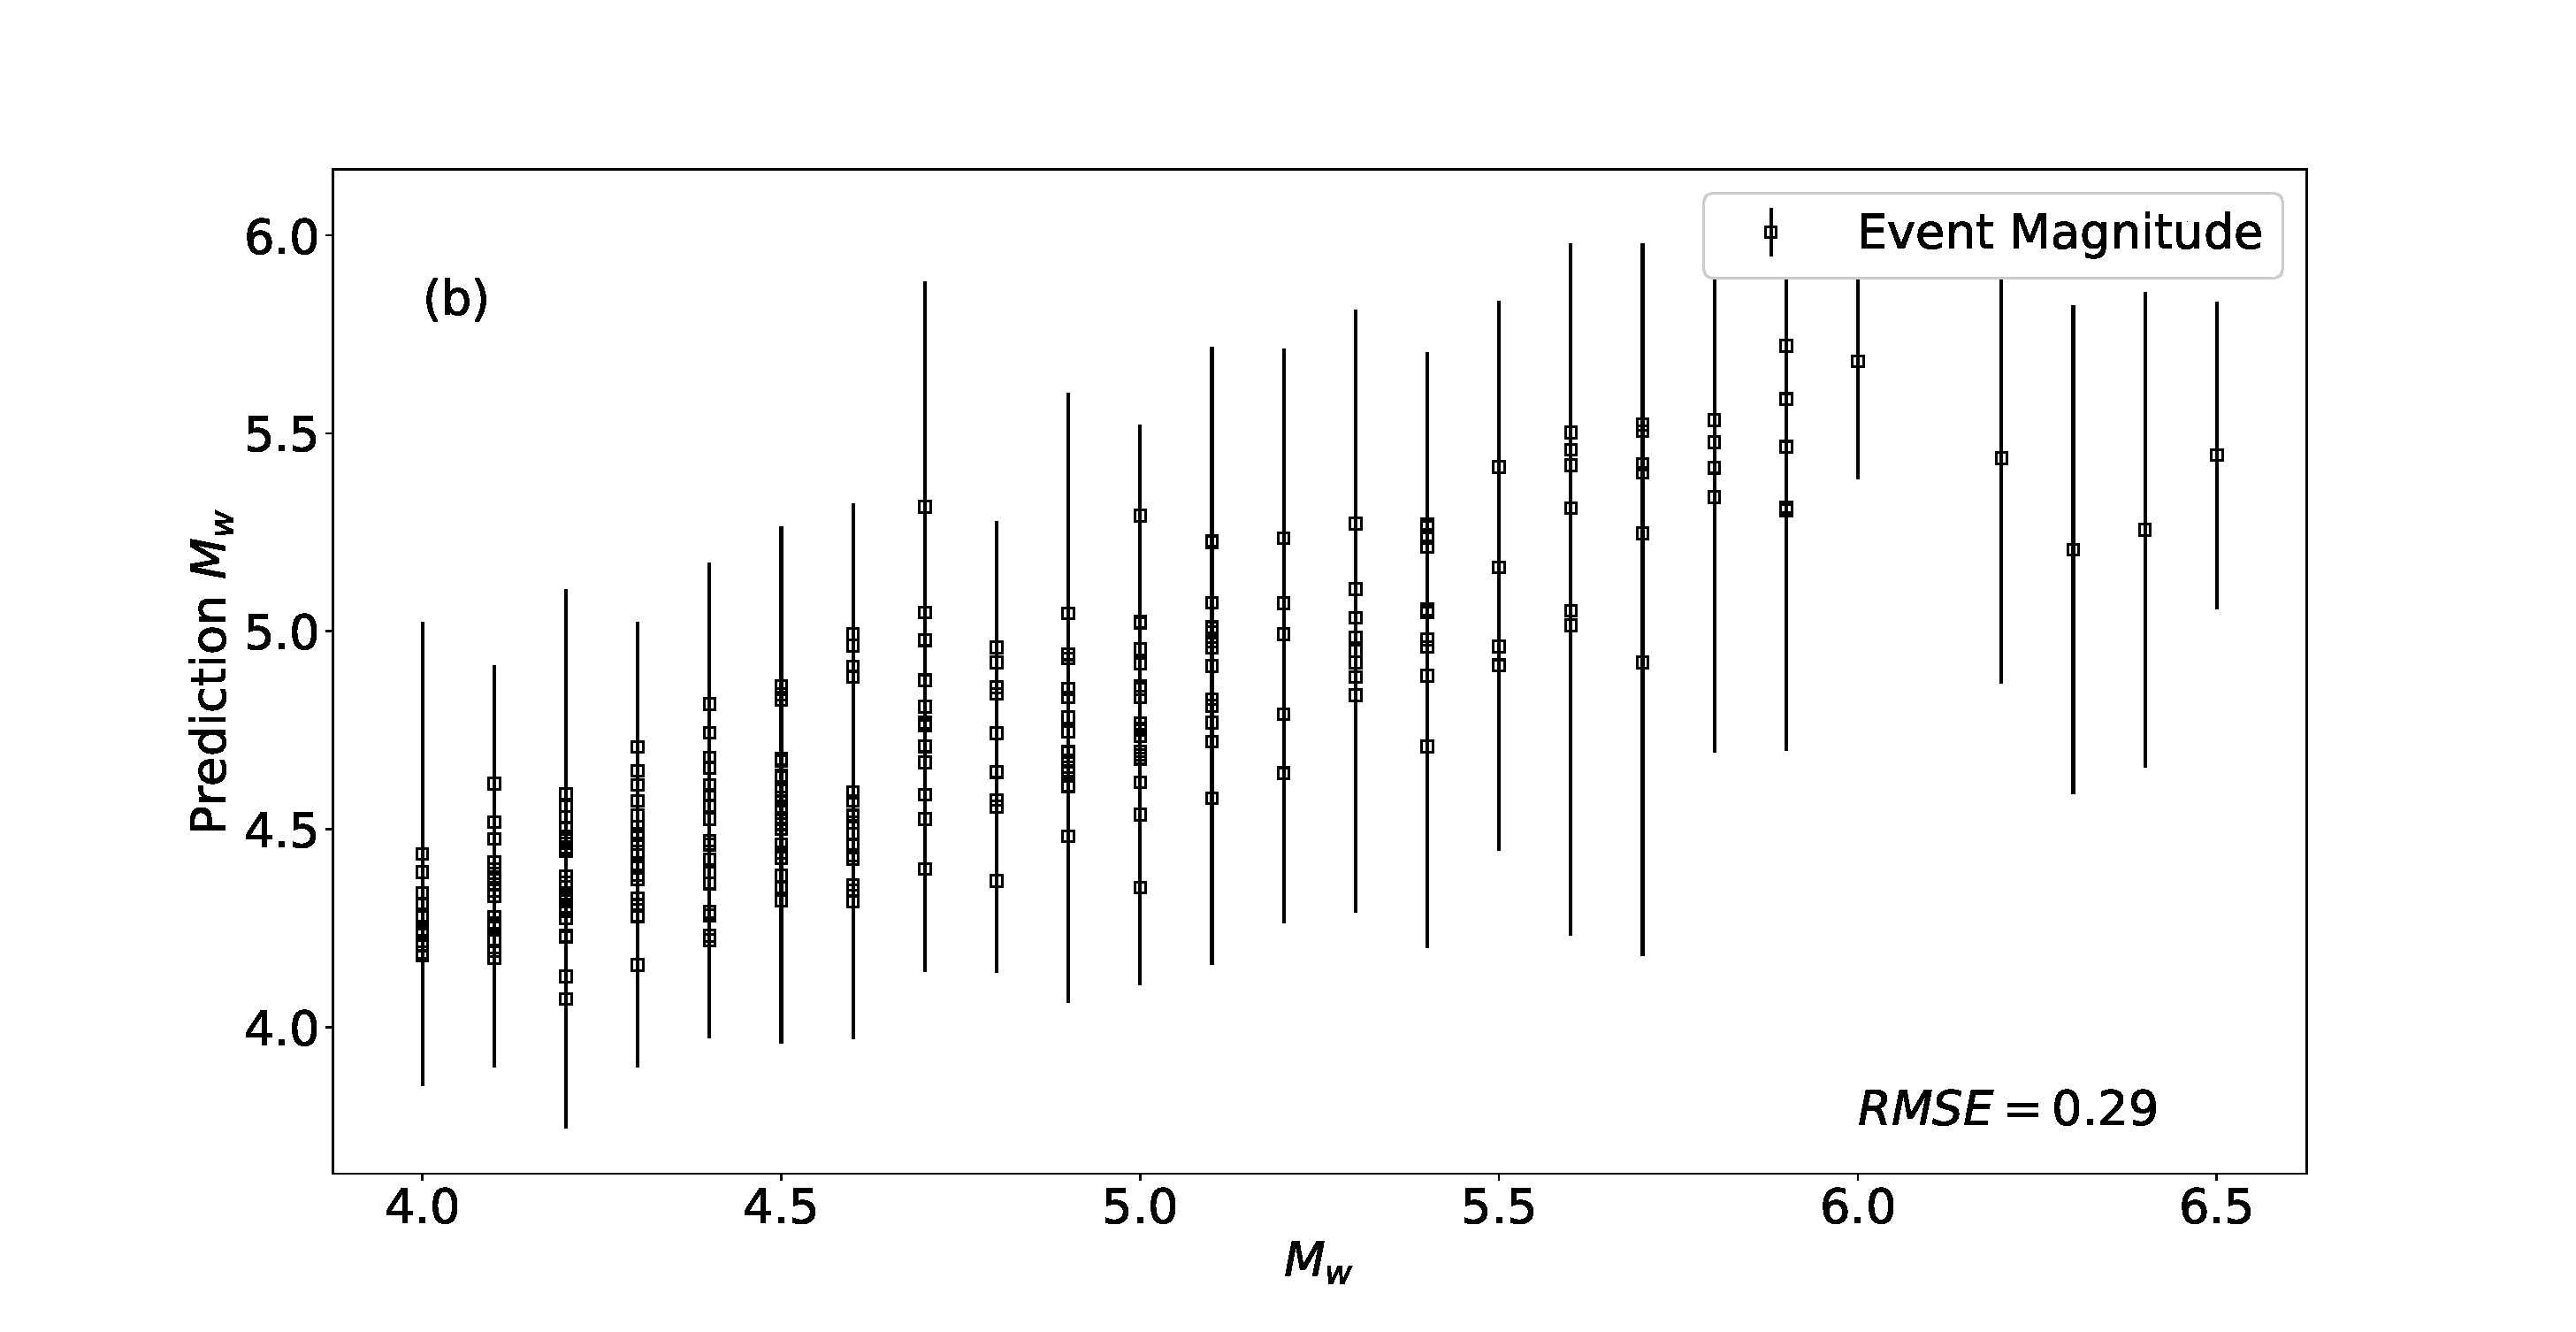
\includegraphics[width=\linewidth]{img/7b.eps}
    \caption{应力影响传播图像}\label{fig:yinglichuanbotuxiang}
  \end{subfigure}
  \caption{应力传播分区图}
\end{figure}


 \begin{figure}[ht]
  \centering
  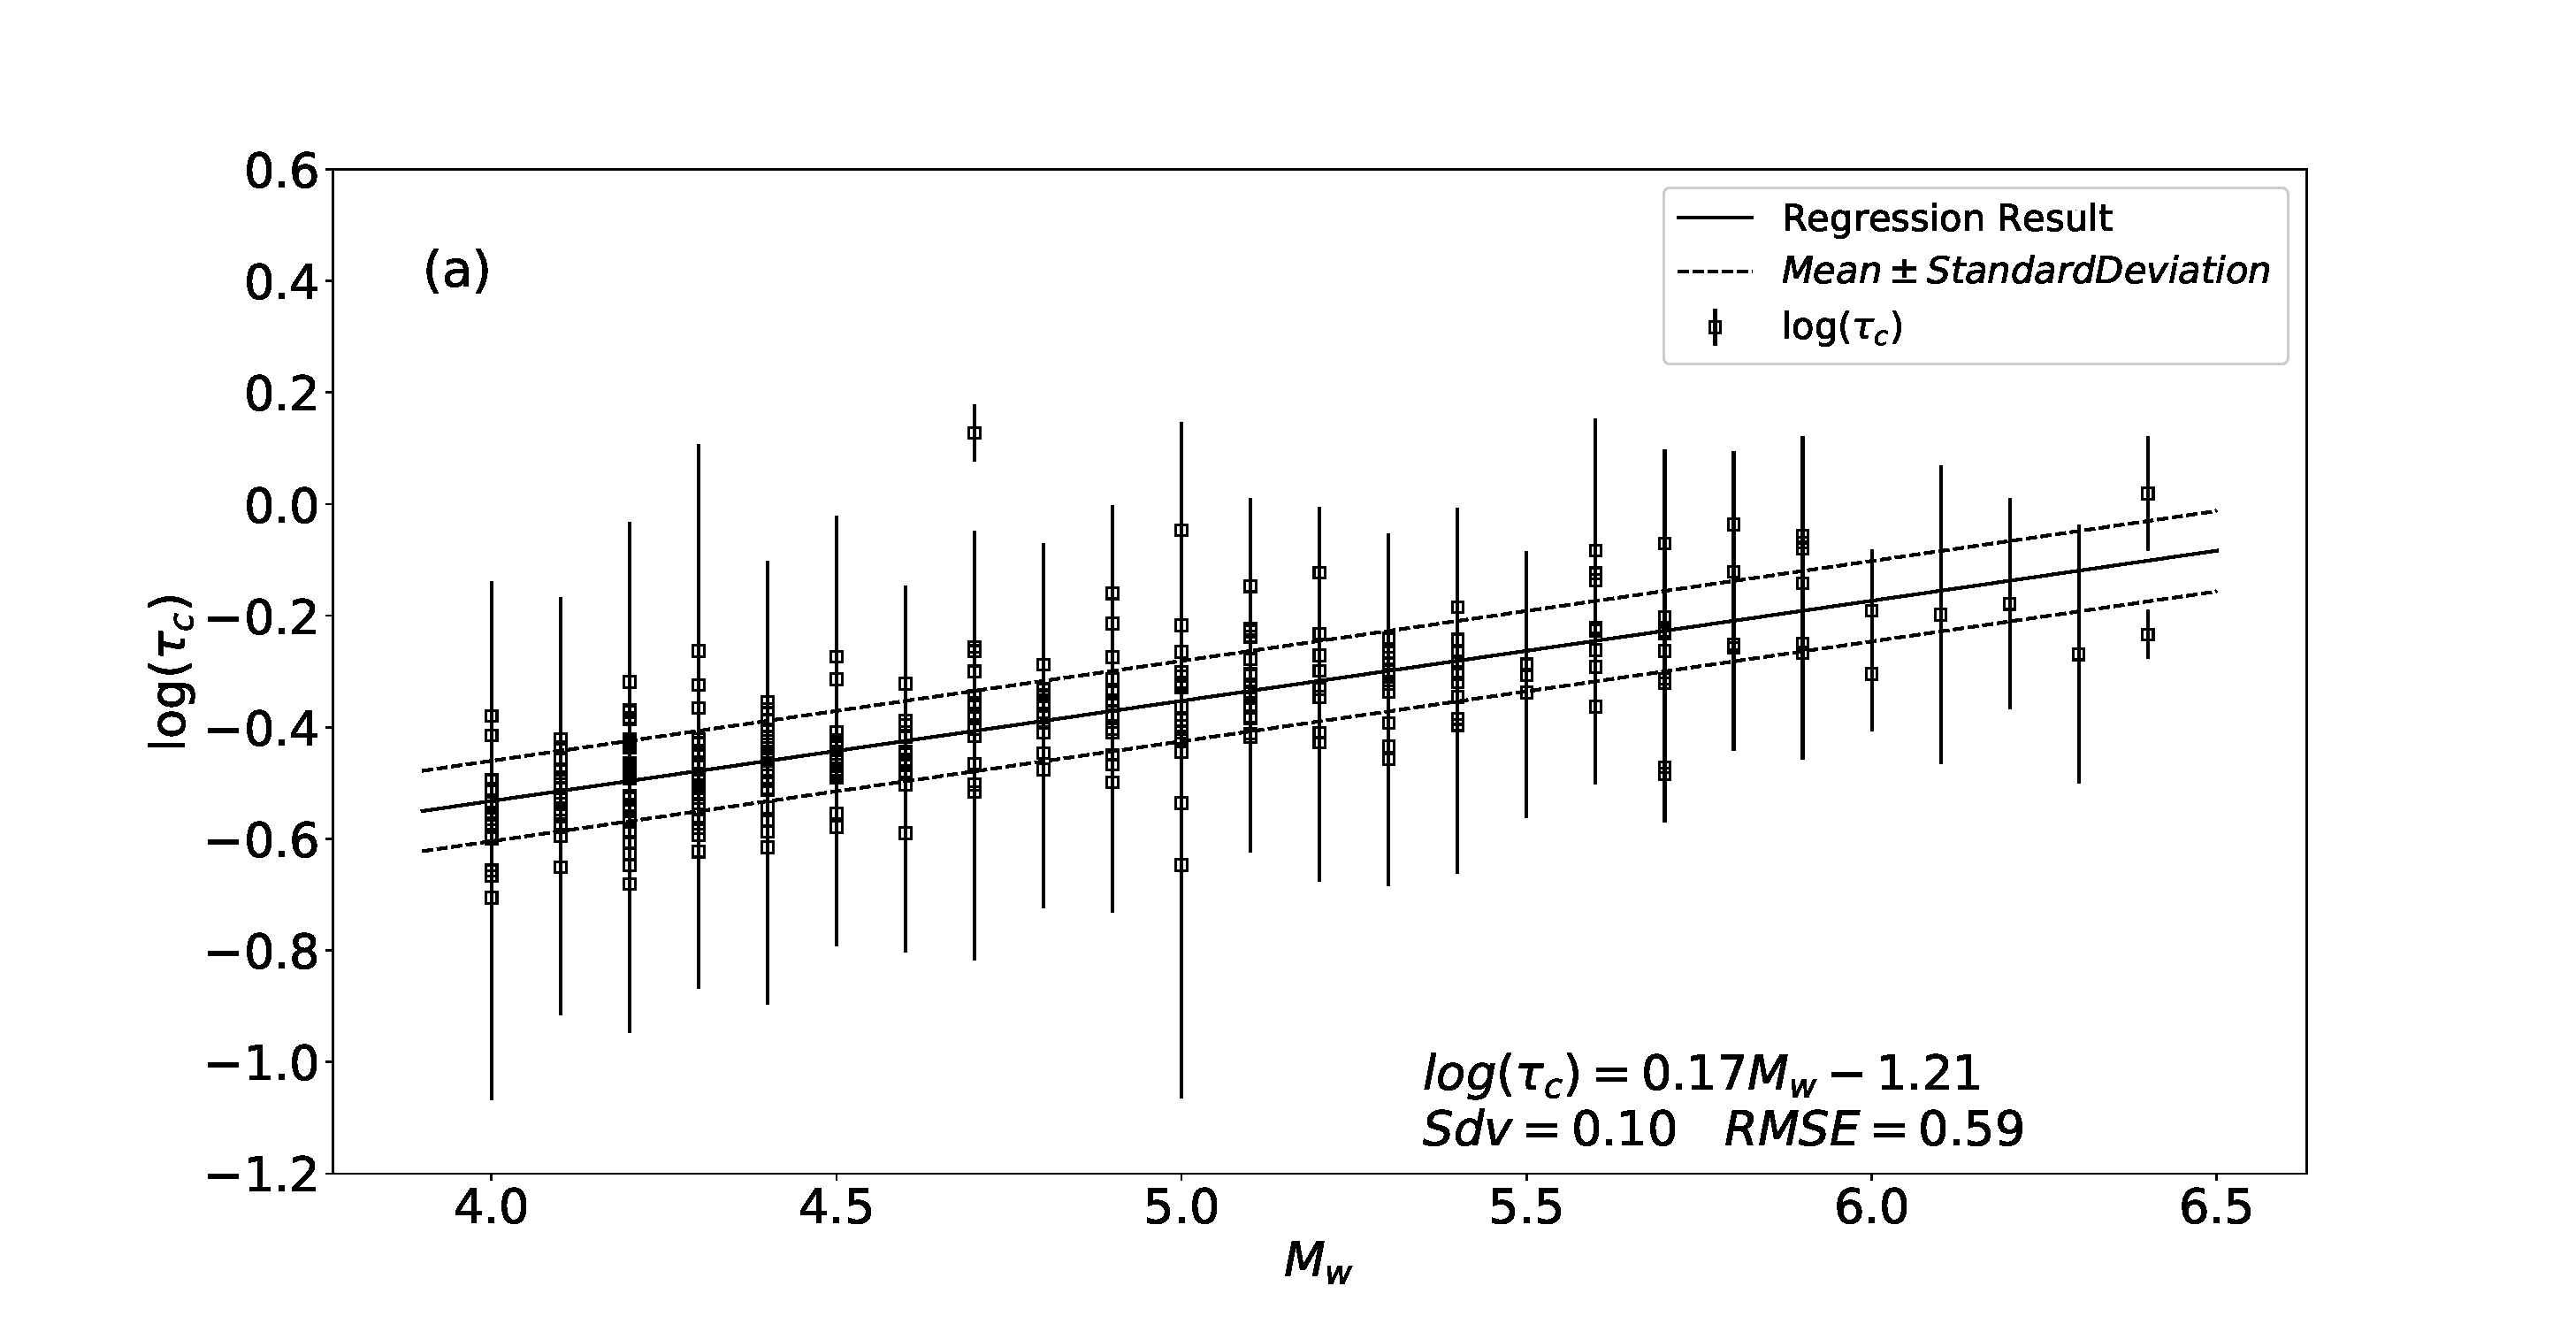
\includegraphics[width=\linewidth]{img/7a.eps}
  \caption{K折交叉检验示意图}\label{fig:yinglimoxin}
\end{figure}

 \begin{figure}[ht]
  \centering
  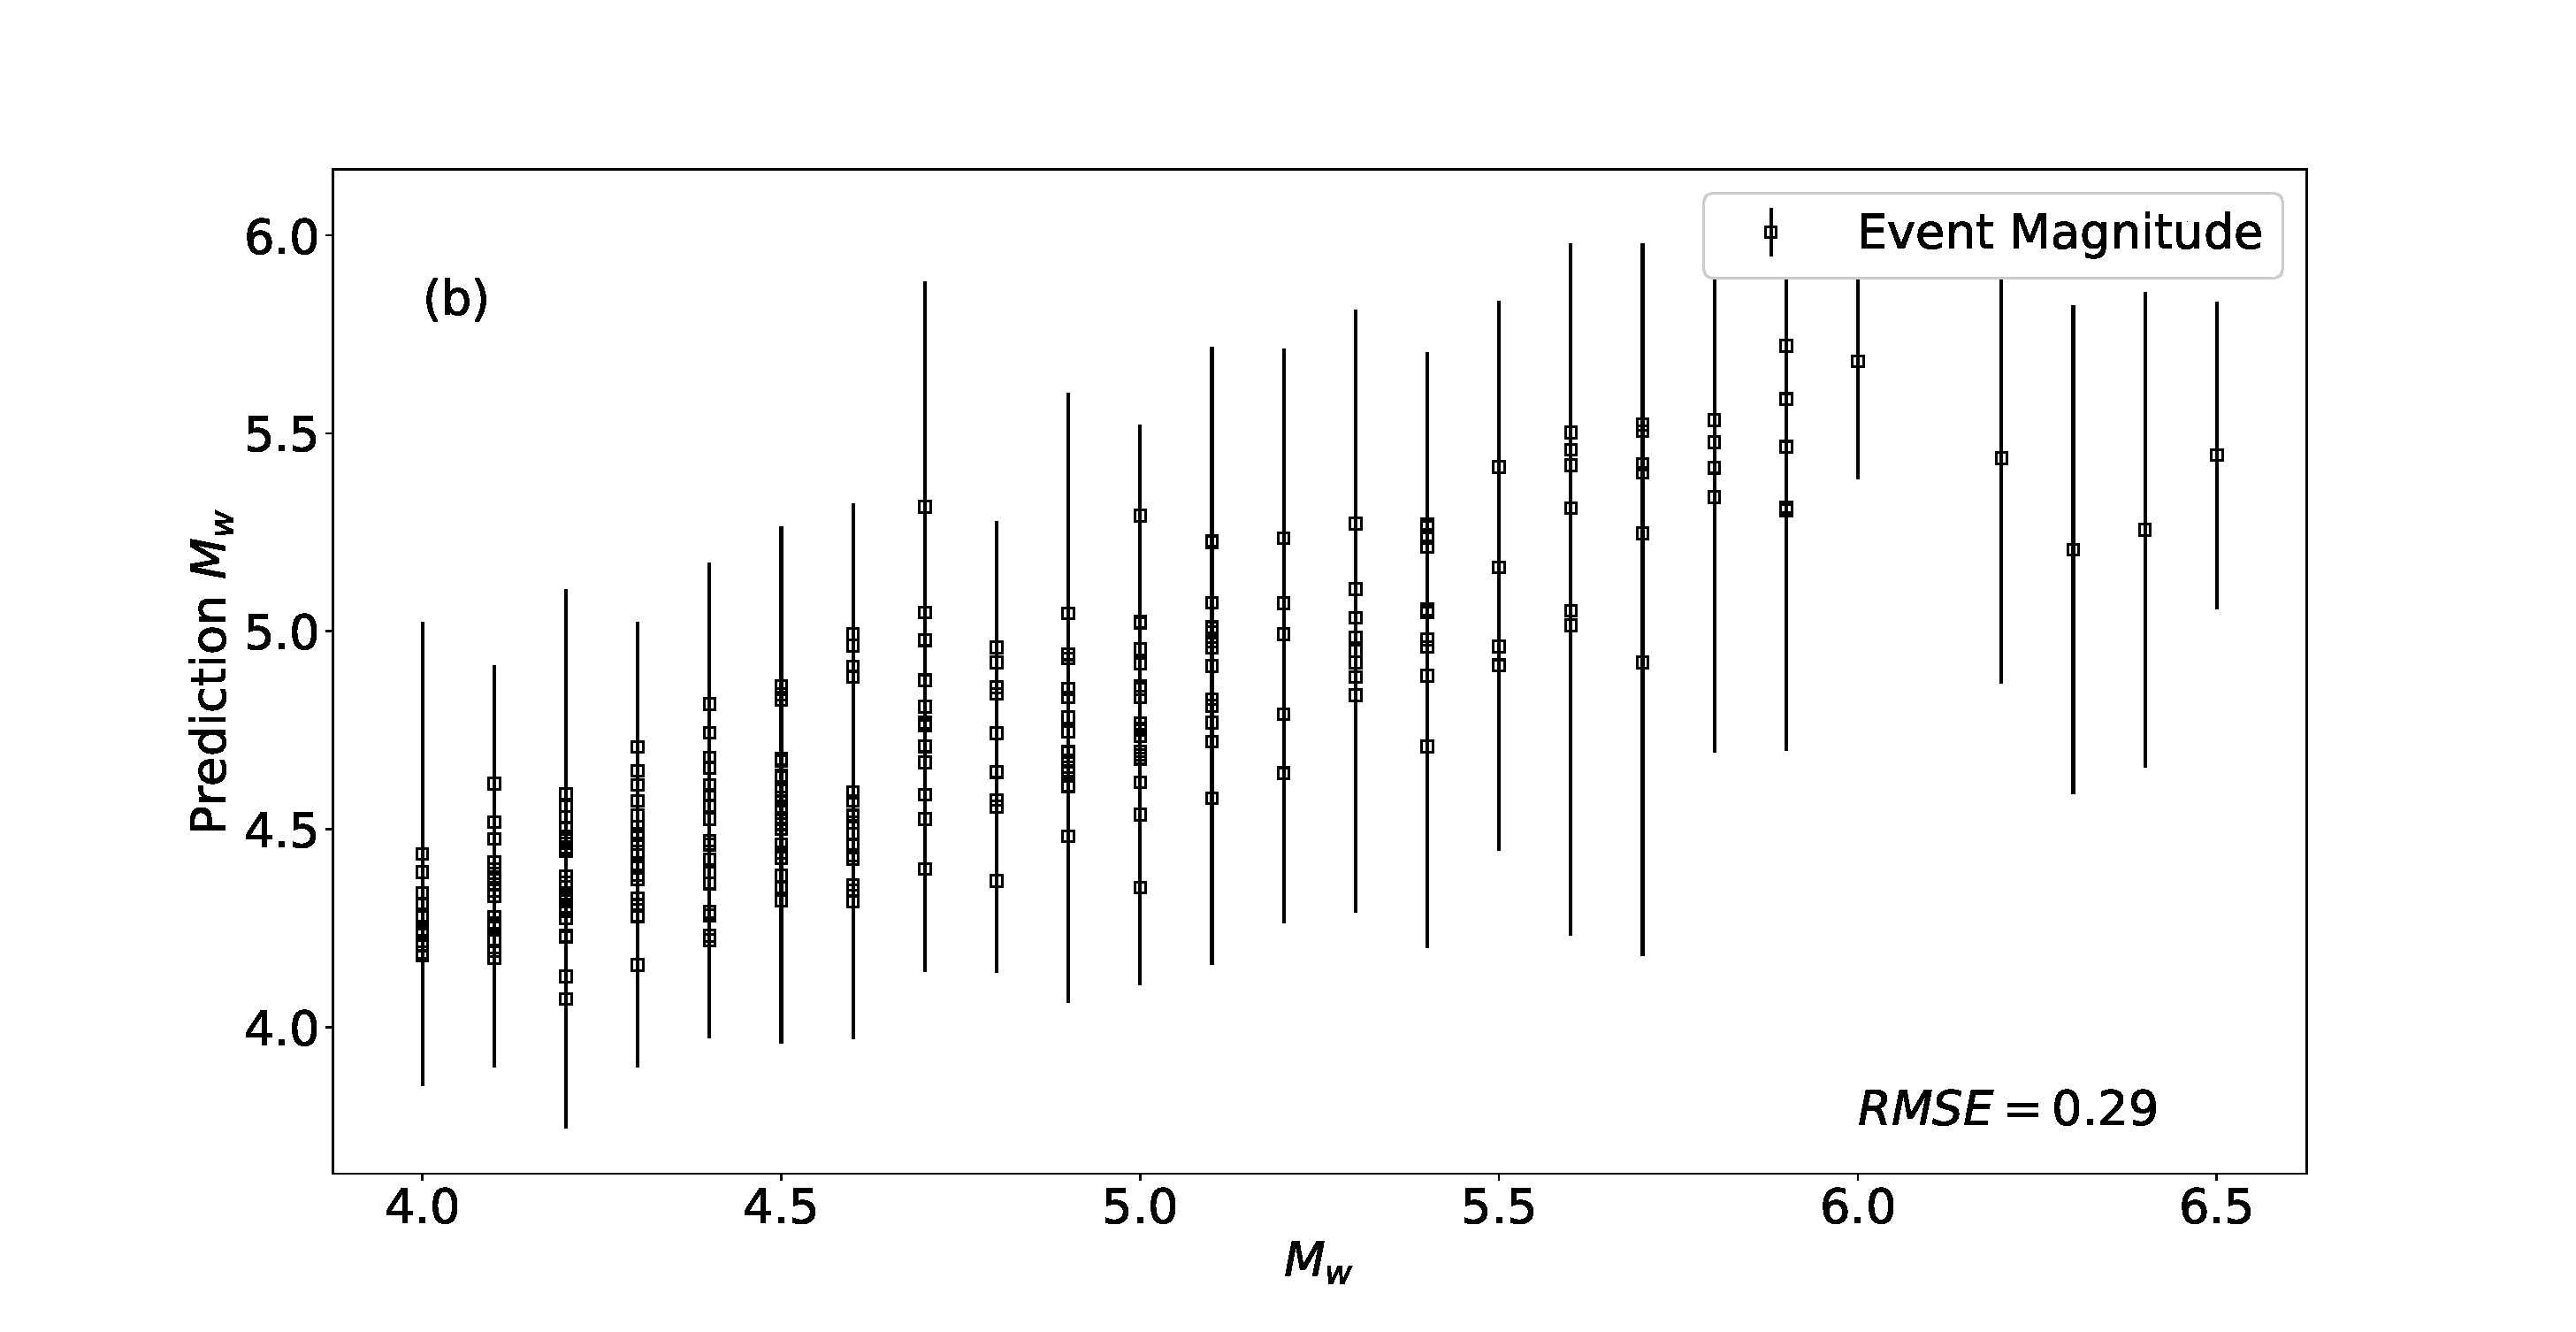
\includegraphics[width=\linewidth]{img/7b.eps}
  \caption{K折交叉检验示意图}\label{fig:yinglimoxin}
\end{figure}



